% Вычислительные эксперименты (
% 1 раздел -- тестирование каждого отдельного метода на предмет скорости сходимости и качества полученного результата, можно сравнить со встроенными функциями sk-learn(?),
% 2 раздел -- тестирование на задаче ИАД,
% 3 раздел -- анализ и комментарии

\newpage
\chapter{Вычислительные эксперименты}





\section{Вычислительный эксперимент на плотных данных малой размерности}

Терм-документная матрица представляет собой матрицу, описывающую частоту терминов,
которые встречаются в коллекции документов.
Рассмотрим следующую подборку из пяти документов \cite{elden}.
Ключевые слова, которые мы называем терминами,
выделены жирным шрифтом.

\begin{longtable*}{ l p{12cm} }
 Документ 1: & The \textbf{Google} \textbf{matrix} $P$ is a model of the \textbf{Internet}. \\
 Документ 2: & $P_{ij}$ is nonzero if there is a \textbf{link} from \textbf{Web} \textbf{page} $j$ to $i$.\\
 Документ 3: & The \textbf{Google} \textbf{matrix} is used to \textbf{rank} all \textbf{Web} \textbf{pages}.\\
 Документ 4: & The \textbf{ranking} is done by solving a \textbf{matrix} \textbf{eigenvalue} problem.\\
 Документ 5: & \textbf{England} dropped out of the top 10 in the \textbf{FIFA} \textbf{ranking}.\\
\end{longtable*}

Если мы посчитаем частоту терминов встречающихся в каждом документе, мы получим следующий результат:

% \begin{center}
 \begin{longtable}{ l | c c c c c c }
 Термин      & Док 1 & Док 2 & Док 3 & Док 4 & Док 5 \\
 \hline
 eigenvalue  & 0 & 0 & 0 & 1 & 0 \\
 England     & 0 & 0 & 0 & 0 & 1 \\
 FIFA        & 0 & 0 & 0 & 0 & 1 \\
 Google      & 1 & 0 & 1 & 0 & 0 \\
 Internet    & 1 & 0 & 0 & 0 & 0 \\
 link        & 0 & 1 & 0 & 0 & 0 \\
 matrix      & 1 & 0 & 1 & 1 & 0 \\
 page        & 0 & 1 & 1 & 0 & 0 \\
 rank        & 0 & 0 & 1 & 1 & 1 \\
 Web         & 0 & 1 & 1 & 0 & 0 \\
 \caption{Терм-документная матрица}
\end{longtable}

Каждый документ можно представить в виде вектора из пространства $\RR^{10}$
Составим из этих векторов матрицу.

\newpage

Ниже приведён полученный результат в виде матрицы $A$:
\begin{equation*}
A =
\begin{pmatrix}
0 & 0 & 0 & 1 & 0 \\
0 & 0 & 0 & 0 & 1 \\
0 & 0 & 0 & 0 & 1 \\
1 & 0 & 1 & 0 & 0 \\
1 & 0 & 0 & 0 & 0 \\
0 & 1 & 0 & 0 & 0 \\
1 & 0 & 1 & 1 & 0 \\
0 & 1 & 1 & 0 & 0 \\
0 & 0 & 1 & 1 & 1 \\
0 & 1 & 1 & 0 & 0
\end{pmatrix}
\end{equation*}

Теперь вычислим неотрицательную факторизацию ранга $k=3$ для данной матрицы.


\subsection{Результат}

График показывает зависимость $f(W, H)$ от номера итерации.

\begin{figure}[h]
  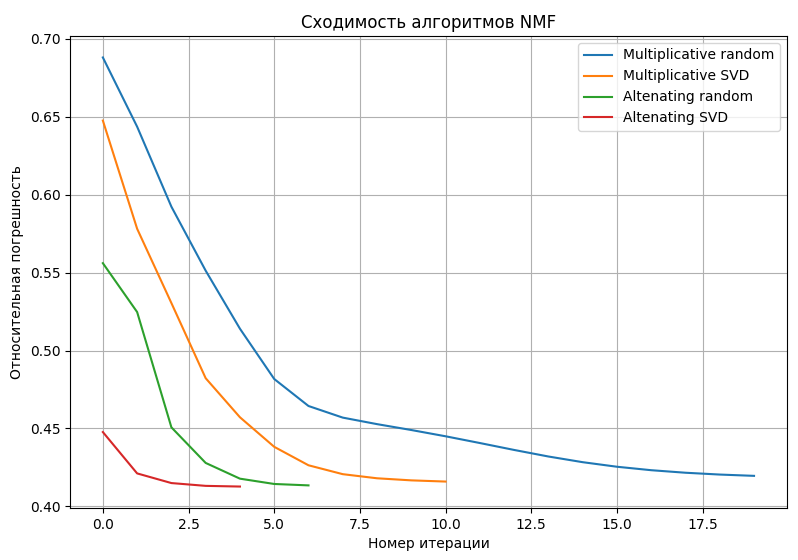
\includegraphics[width=\linewidth]{assets/Graph1.png}
  \caption{График относительной погрешности}
  \label{fig:relativeApproximationError}
\end{figure}

\newpage


Ниже приведены данные показывающие затраты по времени на выполнение алгоритмов:
\\

\begin{lstlisting}[caption=Затраты по времени на выполнение алгоритмов]
# Initialization:
Random takes 2.002e-05s
SVD takes 4.435e-04s
# Methods:
Multiplicative random takes 3.202e-03s
Multiplicative SVD takes 6.939e-04s
Altenating random takes 1.151e-02s
Altenating SVD takes 6.742e-03s
\end{lstlisting}

Ниже приведены результаты алгоритма попеременных наименьших квадратов с использованием SVD инициализации:

\begin{align*}
W H =
\begin{pmatrix}
     0.153  &   0  &   0.089 \\
     0  &   0  &   0.518 \\
     0  &   0  &   0.518 \\
     0.372  &   0.099  &   0 \\
     0.237  &   0  &   0 \\
     0  &   0.516  &   0 \\
     0.525  &  	0  &   0.027 \\
     0.042  &   0.752  &   0 \\
     0.229  &   0.131  &   0.613 \\
     0.042  &   0.752  &   0
\end{pmatrix}
\begin{pmatrix}
     2.152  &   0  &   1.897  &   1.530  &  0 \\
     0  &   1.472  &   1.022  &   0  &   0 \\
     0  &   0  &   0.250  &   0.493  &   1.844
\end{pmatrix}
\end{align*}



\newpage



Полученные данные можно интерпретировать в виде следующих таблиц:

\begin{center}
 \begin{tabular}{ l | c c c c c c }
 Термин      & 1 & 2 & 3 \\
 \hline
 eigenvalue  & 0.153  &   0  &   0.089 \\
 England     & 0  &   0  &   0.518 \\
 FIFA        & 0  &   0  &   0.518 \\
 Google      & 0.372  &   0.099  &   0 \\
 Internet    & 0.237  &   0  &   0 \\
 link        & 0  &   0.516  &   0 \\
 matrix      & 0.525  &  	0  &   0.027 \\
 page        & 0.042  &   0.752  &   0 \\
 rank        & 0.229  &   0.131  &   0.613 \\
 Web         & 0.042  &   0.752  &   0
\end{tabular}
\end{center}

\begin{center}
 \begin{tabular}{ l | c c c c c c }
 Вектор      & Док 1 & Док 2 & Док 3 & Док 4 & Док 5 \\
 \hline
 1           & 2.152  &   0  &   1.897  &   1.530  &  0 \\
 2           & 0  &   1.472  &   1.022  &   0  &   0 \\
 3           & 0  &   0  &   0.250  &   0.493  &   1.844 \\
\end{tabular}
\end{center}

\newpage

\subsection{Вывод}

На Рис.~\ref{fig:relativeApproximationError} отчётливо видно,
что мультипликативным алогритмам необходимо в 2-3 раза больше итераций, чтобы добиться заданной точности.
Также график показывает, что мультипликативные алгоритмы чаще сходятся к более \say{плохой} точке локального минимума,
которая даёт меньшую точность разложения.
Касательно алгоритмов попеременных наименьших квадратов видно, что даже после первой итерации
относительная ошибка значительно меньше чем у предыдущих алгоритмов и в целом они требуют намного меньше итераций.

В обоих случаях инициализация матриц $W$ и $H$ с помощью сингулярного разложения понижает ошибку на первой итерации и уменьшает количество итерации.

Напомним, что первые четыре документа рассказывают о Google и рейтинге веб-страниц,
а пятый касается футбола. Из таблиц можно увидеть, что первые четыре документа представлены векторами,
которые имеют большие компоненты для ключевых слов, связанных с Google.
В отличие от этого, пятый документ представлен только третьим базисным вектором, так же с большой компонентой.
Мы видим, что третий вектор представляет документы рассказывающие о футболе, а два других показывают документы, связанные с Google.






\newpage





\section{Вычислительные эксперименты на разреженных данных}

\subsection{Эксперимент 1}

Для тестирования алгоритмов на больших разреженных данных
было построено разложение ранга $k = 25$ с использованием терм-документной матрицы размера $6947 \times 3837$,
построенной на основе романа \say{Пикник на обочине}.
В критерии остановки итераций \eqref{eq:termination} $\epsilon = 10^{-3}$.

\begin{tikzpicture}[
  trim axis left,
  every mark/.append style={mark size=4pt},
]
  \begin{axis}[
    axis lines = left,
    scale only axis,
    grid = major,
    title = График сходимости алгоритмов,
    xlabel = Номер итерации,
    ylabel = Ошибка,
    width = 0.9\textwidth,
    height = 0.7\textwidth,
    enlarge x limits={0.05},
    enlarge y limits={0.05},
    line width=1pt,
  ]

    \addplot table [
      x=iteration,
      y=roadside_picnic.25.ALS_LSQR,
      col sep=comma,
      skip coords between index={0}{1},
    ] {../samples/data.csv};
    \addlegendentry{ALS\_LSQR - 639s}

    \addplot table [
      x=iteration,
      y=roadside_picnic.25.ALS_NNLS,
      col sep=comma,
      skip coords between index={0}{1},
    ] {../samples/data.csv};
    \addlegendentry{ALS\_NNLS - 412s}

    \addplot table [
      x=iteration,
      y=roadside_picnic.25.ALS_NORM,
      col sep=comma,
      skip coords between index={0}{1},
    ] {../samples/data.csv};
    \addlegendentry{ALS\_NORM - 0.5s}

    \addplot table [
      x=iteration,
      y=roadside_picnic.25.MU,
      col sep=comma,
      skip coords between index={0}{1},
    ] {../samples/data.csv};
    \addlegendentry{MU - 0.7s}

  \end{axis}
\end{tikzpicture}

\begin{itemize}
  \item ALS\_LSQR - Метод попеременных наименьших квадратов на основе алогитма LSQR
  \item ALS\_NNLS - Метод попеременных неотрицательных наименьших квадратов
  \item ALS\_NORM - Метод попеременных наименьших квадратов на основе нормальных уравнений
  \item MU - Метод мультипликативного обновления
\end{itemize}

В виду резкого снижения погрешности после первой итерации, на графиках сходимости не указана погрешность нулевого приближения.
В рассматриваемом случае погрешность равна $1024008.859$.

\begin{figure}[h]
  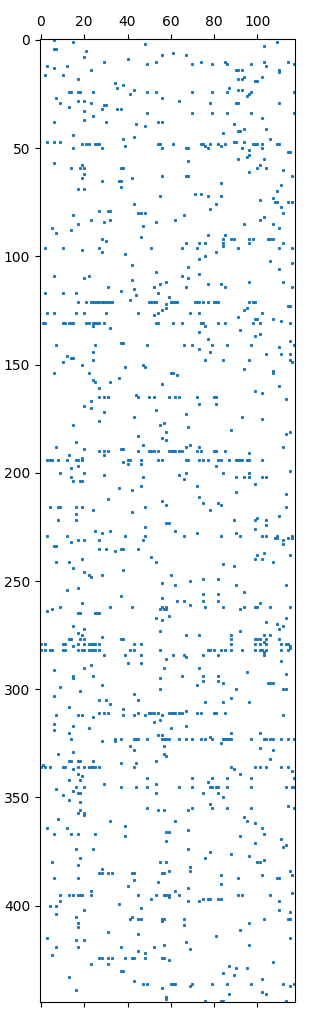
\includegraphics[width=0.3\linewidth]{assets/SparsityPattern.png}
  \caption{Структура разреженности терм-документной матрицы, построенной на основе романа "Пикник на обочине"}
  \label{fig:SparsityPattern}
\end{figure}
\newpage


\subsection{Эксперимент 2}

Следующий график показывает зависимость ошибки получаемого разложения в зависимости от ранга разложения.
Для проведения данного опыта в качестве основы был взят текст первой главы настоящей работы.
Полученная терм-документная матрица состоит из 445 столбцов и 118 строк.
В критерии остановки итераций \eqref{eq:termination} $\epsilon = 10^{-3}$.
Эксперимент проводится с использованием метода попеременных наименьших квадратов на основе нормальных уравнений (ALS\_NORM).

\begin{tikzpicture}[
  trim axis left,
  every mark/.append style={mark size=1pt},
]
  \begin{axis}[
    axis lines = left,
    scale only axis,
    grid = major,
    title = График зависимости ошибки от ранга,
    xlabel = Ранг,
    ylabel = Ошибка,
    width = 0.9\textwidth,
    height = 0.7\textwidth,
    enlarge x limits={0.05},
    enlarge y limits={0.05},
    line width=1pt,
  ]

    \addplot table [
      x=rank,
      y=error,
      col sep=comma,
    ] {../samples/rank-error.csv};

  \end{axis}
\end{tikzpicture}

\newpage

\subsection{Выводы}

Эксперимент 1 показывает, что метод попеременных неотрицательных наименьших квадратов (ALS\_NNLS)
сходится к самому \say{лучшему} приближению, так как каждый шаг неотрицательных наименьших квадратов
не требует дополнительного проецирования результата на неотрицательную область.
Однако метод требует большое количество вычислительных ресурсов, так как шаги неотрицательных наименьших квадратов
не приспособлены к работе с большими разреженными матрицами.

Самым эффективным методом среди рассмотренных является метод попеременных наименьших квадратов на основе нормальных уравнений,
так как данный метод даёт \say{достаточно хорошее} приближения за наименьшее время.

Эксперимент 2 показывает, что при увеличении ранга $k$ аппроксимации методы начинают сходиться к более \say{глубоким} локальным минимумам.
Это можно объяснить тем, что при аппроксимации малым рангом происходит некоторое \say{сжатие} данных или выделение \say{важных} данных, и чем больше ранг аппроксимации,
тем легче методам сойтись к более \say{глубокому} локальному минимуму.

\newpage





\section{Вычислительный эксперимент на задачах интеллектуального анализа текста}

Для проведения данного опыта в качестве основы взят текст первой главы настоящей работы.
Для каждой рассмотренной задачи проведено выделение 5 ключевых предложений.
Анализ результата проведём в следующей секции.


\subsection{Результат метода оценки значимости}

\begin{itemize}
  \item Ключевой характеристикой неотрицательной матричной факторизации является возможность
  использования численных методов для минимизации \eqref{eq:min_problem}
  для извлечения некоторых базовых признаков в качестве базисных векторов матрицы $W​$,
  которые затем могут быть использованы для поиска и классификации.
  \item Несмотря на многие недостатки неотрицательная матричная факторизация весьма привлекательна для приложений интеллектуального анализа данных,
  поскольку на практике даже локальные минимумы могут обеспечивать желаемые свойства, такие как сжатие данных и извлечение базовых признаков.
  \item Эта блокировка нулевых элементов является большим ограничением алгоритма,
  что означает как только алгоритм начинает двигаться вниз по пути к фиксированной точке,
  даже если это \say{плохая} фиксированная точка, алгоритм продолжит двигаться в направлении к этой точке.
  \item Численные методы решения задачи неотрицательной матричной факторизации могут быть поделены на следующие основные категории: 	Методы мультипликативного обновления, 	Методы попеременных наименьших квадратов, 	Методы градиентного спуска.
  \item Стоит отметить что все вышеперечисленные методы решают задачу неотрицательной матричной факторизации,
однако название \textit{"метод неотрицательной матричной факторизации"} обычно применимо только к методам решающим задачу в формулировке \eqref{eq:min_problem}.
\end{itemize}


\newpage


\subsection{Результат метода извлечение ключевых предложений из аппроксимации ранга $k = 5$}

\begin{itemize}
  \item Эта блокировка нулевых элементов является большим ограничением алгоритма,
  что означает как только алгоритм начинает двигаться вниз по пути к фиксированной точке,
  даже если это \say{плохая} фиксированная точка, алгоритм продолжит двигаться в направлении к этой точке.
  \item Ниже будет использован несколько модифицированный вариант нормы Фробениуса, который будем называть относительной погрешностью нормы Фробениуса.
  \item  Ключевой характеристикой неотрицательной матричной факторизации является возможность
  использования численных методов для минимизации \eqref{eq:min_problem}
  для извлечения некоторых базовых признаков в качестве базисных векторов матрицы $W​$,
  которые затем могут быть использованы для поиска и классификации.
  \item Несмотря на многие недостатки неотрицательная матричная факторизация весьма привлекательна для приложений интеллектуального анализа данных,
  поскольку на практике даже локальные минимумы могут обеспечивать желаемые свойства, такие как сжатие данных и извлечение базовых признаков.
  \item Численные методы решения задачи неотрицательной матричной факторизации могут быть поделены на следующие основные категории: 	Методы мультипликативного обновления, 	Методы попеременных наименьших квадратов, 	Методы градиентного спуска.

\end{itemize}

\newpage

\subsection{Выводы}

Метод, основанный на оценках значимости, имеет недостаток:
если в тексте присутствуют два и более \say{самых значимых предложения}, которые содержат одинаковые термы высокой значимости,
то их координаты будут примерно одинаковыми, и оба предложения будут извлечены как ключевые.
Но это не практично со стороны поиска информации, так как они очень похожи.

По результатам видно, что оба метода предпочитают более длинные предложения.

Также по результатам можно понять, что метод извлечение ключевых предложений из
аппроксимации ранга $k$ старается включить в выборку предложения касающиеся \say{ортогональных} тем.
Под \say{ортогональностью} тем подразумевается их разнородность и в некоторой мере субъективная оценка.
Такие свойства метода напрямую вытекают из использования $QR$ разложения.

Учитывая всё вышесказанное, можно сделать вывод, что метод извлечение ключевых предложений из
аппроксимации ранга $k$ даёт более качественную выборку, однако требует больше вычислительных ресурсов.
